\section{The Mechanics and Pragmatics of Lifespan Development: Conceptualization, Measurement and Plasticity}
\shorttitle{Mechanics and Pragmatics of Lifespan Development}

According to modern notions of development such as the lifespan approach, human development is the result of the interaction between three different sources: biology (maturation/senescence), culture (learning), and an individual (decision/action). It is further assumed that psychological phenomena can be meaningfully and for heuristic purposes distinguished in those of the life mechanics and those of the life pragmatics (e.g., Staudinger \& Pasupathi, 2000). Life mechanics reflect individual differences in biology-based patterns of perception, information processing, emotion, and motivation (e.g., basic motivational (approach/avoidance) and emotional (positive/negative) patterns, temperament, speed of information processing, executive processes). Life pragmatics reflect individual differences in the accumulated and constructed experiences with the world (i.e., other people, events, circumstances, rules, places, and objects relevant for leading our lives) and with our self, as well as ways of dealing with the world and with ourselves (e.g., coping, emotion regulation, goal system). In the long run, it seems essential for our understanding of developmental processes to successfully decipher the co- and interaction of those two elements. Presently our research efforts however concentrate on the domain of life pragmatics. Life pragmatics can be distinguished in constructs related to insight and those related to compository or management strategies. With regard to insight, we study insight into life (life insight) as well as insight into our self (self-insight) and the highest form of both, that is, wisdom. With regard to compository strategies, we are especially interested in personal life investment, emotion regulation, coping and time experience. 

Life insights as well as life-compository structures and processes are not determined but plastic. Within a 'norm of reaction' better or worse developmental trajectories are conceivable. Given this basic contention of the plasticity of human development, it is crucial to determine the conditions of plasticity as well as its limits in different domains of psychological functioning. Thus, a third and fourth research focus concern themselves with the theoretical and empirical investigation of the plasticity of human development. The third focus concentrates on the effects of (in particular social) contexts on adult development and the fourth focus is primarily theoretical in nature. It explores the question of different types of plasticity, such as growth and resilience, and pursues the thesis that it is useful to distinguish two different kinds of positive adult development, one aiming towards growth and the other geared towards adjustment. In the following, these four research foci are described in turn.

\textbf{Central reference} Staudinger, U. M. \& Pasupathi, M. (2000). Lifespan perspectives on self, personality and social cognition. In T. A. Salthouse \& F. I. M. Craik (Eds.), The handbook of aging and cognition (pp. 633-688). Hillsdale, NJ: Erlbaum.

\subsection{Life Insight, Self Insight, and
Wisdom: Measurement, Age Trajectories}


\index{Staudinger, M. Ursula}

\paragraph{Research Team}
Ursula M. Staudinger (Professor), Jessica D\"orner (Doctoral Fellow; graduated 05/2006; postdoctoral fellow until 08/2006).

Life insight, and in particular wisdom as its highest form, represent the prototype of growth in adulthood. One may think that such phenomena defy empirical study. But a reliable and valid measurement paradigm has been developed (Baltes \& Staudinger, 2000). Consistent with cultural-historical writings about wisdom, there is empirical evidence that wisdom is indeed a phenomenon that depends on the successful integration of mind and character (Staudinger, Lopez, \& Baltes, 1997). The analysis and evaluation of important life experiences play an important part in that integration process. Thus, it does not come as a surprise that it is not enough to grow older to become wiser. In the last two years, a differentiation between personal wisdom and self-insight on the one and general wisdom and life insight on the other hand has been introduced and a measurement paradigm has been developed. This distinction is based on the assumption that distinguishable psychological phenomena are concerned when you have to be wise about a problem of your own life or life in general.

\null
\textbf{Research Highlights 2006}

Using the two new measures of self-insight or personality maturity that had been developed before, we started to investigate their age trajectories during the last year. As expected, based on the literature on personality growth, we found that neither self-related wisdom nor self-concept maturity normatively show positive age differences. In terms of self-related wisdom, we even found negative age differences in particular with regard to the three meta criteria of self-related wisdom, that is, tolerance, embeddedness and tolerance of ambiguity. This finding is consistent with the interpretation that the last developmental task of life, that is, integrating our lives and finding peace in the face of human terminality, may be juxtaposed to the goal of pursuing self-related wisdom.

\paragraph{Collaborations}

\begin{itemize}
\item Max Planck Institute for Human Development, Berlin\\ Prof. Dr. Paul B. Baltes ($\dagger$)
\item Oregon State University\\ Prof. Karen Hooker, PhD
\item IUB, JCLL\\ Prof. Dr. Ute Kunzmann
\item IUB, JCLL\\ Prof. Dr. Sven V\"olpel
\item University of Florida, Gainsville, FLA\\ Prof. Manfred Diehl, PhD
\item Universit\"at Frankfurt\\ Prof. Dr. Tilmann Habermas
\item Universit\"at Wien\\ Prof. Dr. Judith Gl\"uck
\end{itemize}

\begin{bibunit}[apalike]
\nocite{*}
\putbib[profUrsulaStaudinger1]
\end{bibunit}

\paragraph{Grants}
\begin{itemize}
\item DFG STA 540/3 -1/2(PI: U.M. Staudinger): Is it possible to promote self-insight? (2001-2005)
\end{itemize}

\subsection{Life Composition: Measurement and Age Trajectories}


\index{Staudinger, M. Ursula}

\paragraph{Research Team}
Team Ursula M. Staudinger (Professor), Eva-Marie Kessler (Doctoral Candidate; graduated 01/2006; postdoctoral fellow), Ines Schindler (Postdoctoral fellow at Utah State University).

This project is interested in processes of developmental regulation during adulthood and old age. Life composition concerns different aspects of self and personality such as emotions, coping, the goal system, and the experience of time. Besides establishing valid measurement for different age groups, we investigate which role these aspects of self and personality play in resilience constellations and the regulation of subjective well-being of old age. 

\null 
\textbf{Research Highlights 2006}

\textit{Personal Life Investment}

 During 2006, work in the area of the goal system (personal life investment, PLI) focused on the distinction between obligatory and optional PLI. PLI is defined as the amount of motivational energy people invest as actions or thoughts in ten central life domains (health, cognitive fitness, hobbies and interests, relationship with friends and acquaintances, sexuality, well-being of relatives, occupation or similar activities, independence, thinking about one's life, death and dying) in order to achieve their personal goals or prevent the loss of prior achievements. Depending on the developmental tasks of a given age period different domains require our obligatory investment and others leave room for optional investments. 

\begin{figure}[htb]
  \begin{center}
    \resizebox{0.4\textwidth}{!}{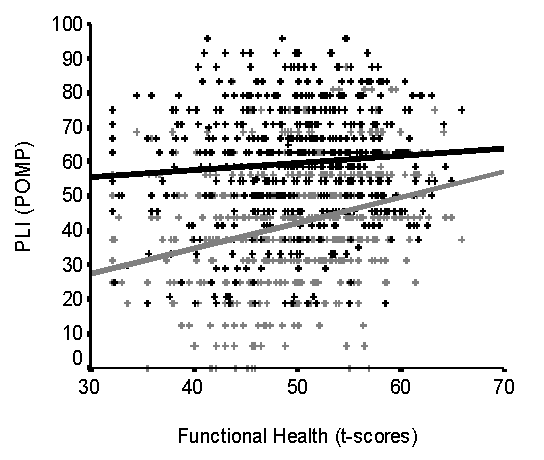
\includegraphics{profUrsulaStaudinger-fig1}}
    \caption{Optional (grey line) and obligatory (black line) as expected differ in their association with levels of objective health. Optional PLI is higher at higher levels of functional health (Schindler \& Staudinger, submitted).}
    \label{fig1:profUrsulaStaudinger}
  \end{center}
\end{figure}


The distinction aims to model the differences between reactive and active types of investments. And indeed, we found that the two types relate differently to indicators of approach and avoidance as well as to indicators of subjective well-being (see Figure \ref{fig1:profUrsulaStaudinger}; Schindler \& Staudinger, submitted). The two types of PLI have demonstrated differential age trajectories in the longitudinal sample of the Berlin Aging Study (Schindler, Staudinger, \& Nesselroade, in press). Across an age range of 30 years and a measurement period of 10 years, optional PLI showed declines and obligatory PLI stayed stable. This finding was replicated when using functional health rather than chronological age as correlate. Obligatory PLI is not related to functional health whereas optional PLI is lower at lower levels of health.

%\begin{figure}[ht]
%  \begin{center}
%    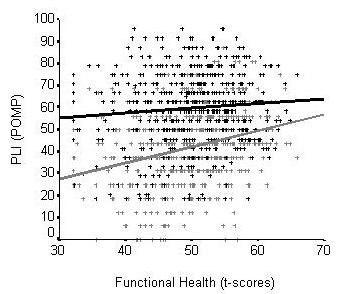
\includegraphics[width=7.5cm]{profUrsulaStaudinger-fig1.png}
%    \caption{Optional (grey line) and obligatory (black line) as expected differ in their association with levels of objective health. Optional PLI is higher at higher levels of functional health (Schindler \& Staudinger, submitted).}\label{fig1:profUrsulaStaudinger}
%   \end{center}
%\end{figure}


Furthermore, in 2006 we conducted a study on the emotional life and its functionality across the lifespan (Kessler \& Staudinger, in preparation). A new emotion questionnaire that assesses the frequency with which certain emotions have been experienced was developed. In contrast to extant questionnaires, the new instrument distinguishes not only between positive and negative emotions but also between emotions that involve high and those that involve low activation. Some of the conflicting patterns of results available in the literature may be related to the lack of this differentiation. And indeed this is what we found: both high and low activated negative emotions decline starting in midlife. Highly activated positive emotions show no age differences, but low activated positive emotions increase starting young adulthood (see Figure \ref{fig2:profUrsulaStaudinger}).

%\begin{figure}[ht]
%  \begin{center}
%    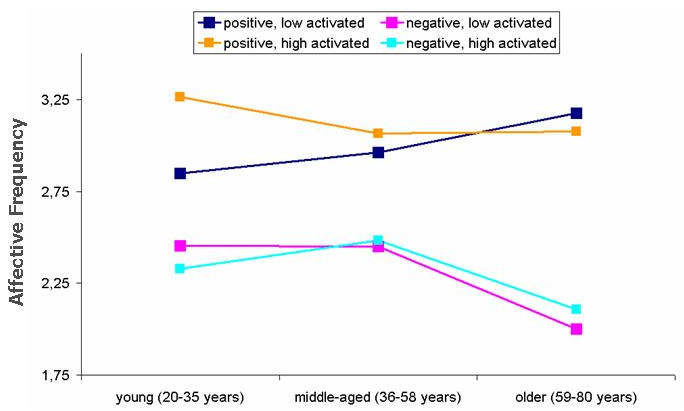
\includegraphics[width=7.5cm]{profUrsulaStaudinger-fig2.png}
%    \caption{Age difference on four facets of emotional life (Kessler \& Staudinger, in preparation).}\label{fig2:profUrsulaStaudinger}
%   \end{center}
%\end{figure}


\begin{figure}[htb]
  \begin{center}
    \resizebox{0.5\textwidth}{!}{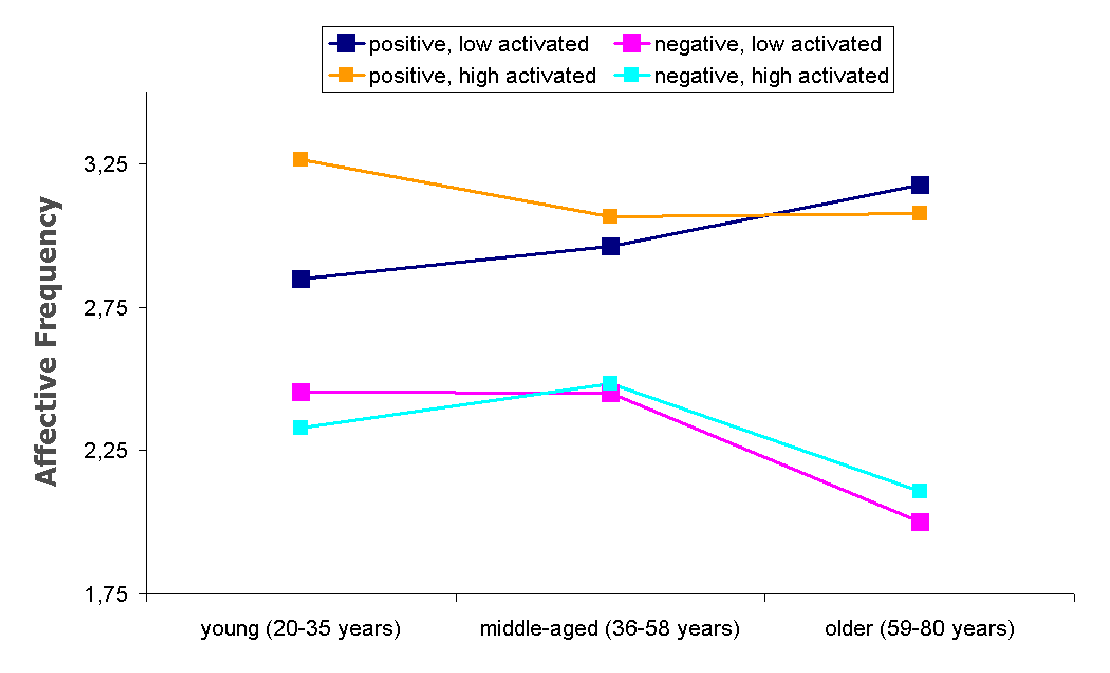
\includegraphics{profUrsulaStaudinger-fig2}}
    \caption{Age difference on four facets of emotional life (Kessler \& Staudinger, in preparation).}
    \label{fig2:profUrsulaStaudinger}
  \end{center}
\end{figure}

\newpage
\paragraph{Collaborations}

\begin{itemize}
\item Brandeis University\\ Prof. Margie Lachman, PhD
\item Stanford University\\ Prof. Laura Carstensen, PhD
\item University Hildesheim\\ Prof. Dr. Werner Greve
\item University of Utah\\ Dr. Ines Schindler
\end{itemize}

\begin{bibunit}[apalike]
\nocite{*}
\putbib[profUrsulaStaudinger2]
\end{bibunit}

\subsection{Context as a Facilitator of Adult Personality
Development}


\index{Staudinger, M. Ursula}

\paragraph{Research Team}
Ursula M. Staudinger (Professor), Heike Heidemeier (Postdoctoral Fellow (since 03/2006), Eva-Marie Kessler (Doctoral Fellow, graduated 01/2006; now Postdoctoral Fellow), Andrea M\"uhlig-Versen (Doctoral Fellow), Martin Noack (Doctoral Fellow since 03/2006).


As mentioned in the Introduction, the plasticity of human development is the third research focus besides the study of life insight and life composition. Plasticity of human development is based on resources. Internal (biological, psychological) and external (contextual) resources can be distinguished. In the present project we are concerned with four different approaches to the study of contextual effects on human development: (1) interactive minds: the facilitative effects of social context; (2) social context and intergenerational potential; (3) activating contexts for old age: the sample case of civic engagement; and (4) the investigation of the effects of the work context on adult development.

\null
\textbf{Research Highlights 2006}

\textit{Interactive Minds}

 In earlier studies on life insight, we had found that under specific conditions (natural partner, time to think after interaction) social interaction facilitates life insight and wisdom (Staudinger \& Baltes, 1996). Furthermore, life-reflection has been identified as a central mechanism in the accumulation of life experience (Staudinger, 2000). We conducted an intervention study that aimed to facilitate self-insight or personality maturity by learning a social-cognitive strategy of how to think about oneself in the present, the past and the future. This strategy is called life-reflection is composed of three elements: (1) remembering experiences, (2) explain experiences, (3) evaluate experiences in the context of one's life. Based on earlier work on interactive minds (Staudinger \& Baltes, 1996), we recruited natural dyads to come to the lab. These dyads were randomly assigned to the following experimental conditions: (1) Life reflection dyad, (2) Life reflection alone, (3) Reminiscence, (4) Thinking time alone. In each of the conditions, participants had to respond to a self-related wisdom task (e.g., how are you as a friend?) either with or without having learnt how to do life reflection and either doing it alone or as a twosome. First results with regard to the new measure of self-related wisdom showed that applying the social-cognitive strategy of life reflection increased self-insight significantly. No significant differences between young and old adults were found neither were there differences between the monadic and the dyadic condition. The lack of a facilitative effect of the natural dyadic condition is in contrast to earlier findings with general wisdom. This finding is consistent with the interpretation that conversational partners that know each other well may not be so helpful when it come to stimulating new self-insight, as mutual perceptive patterns have been established as well as tabu topics to be avoided. The study underscores the importance of the social-cognitive process of life reflection on our way to wisdom (Staudinger, D\"orner, \& Mickler, in preparation).

\textit{Social Context and Intergenerational Potential}

 In this study, funded by the DFG, we investigated the effect of age-heterogeneous interactions between adolescents and older adults on psychological functioning (e.g., fluid intelligence, prosocial behavior). The thesis is that the developmental motivations of adolescents (identity formation/information search) and older adults (generativity) provide for a motivational match that facilitates psychological functioning. For this match to be realized, however, the situational conditions need to be such that both motivations get activated. This hypothesis was confirmed. Older adults that interacted with an adolescent over a difficult life problem (that makes the older person the expert) afterwards show higher levels of cognitive functioning on speed-dependent measures than older adults that interacted with adolescents over a new technology problem (that makes the adolescent the expert; Kessler \& Staudinger, submitted). The assumption was that the motivational match would create a motivational boost that activated in particular those aspects of cognitive functioning that are dependent on cognitive energy such as speed measures. In turn, adolescents in age-heterogeneous interaction over a life problem showed significantly more prosocial behavior than those who had interacted with a peer or with an older adult over a technology problem. 

\textit{Contexts that Activate in Old Age: The Sample~Case of Civic Engagement}

 Funded by the BMFSFJ, we conducted a quasi-experimental longitudinal field study that investigated whether the participation in a special volunteer program (EFI) that combines participation in a preparatory training for volunteering with civic engagement leads to personality changes in older adults. The training program aims to develop a role identity in the area of civic engagement and to teach competences necessary in the realm of civic engagement. The EFI participants were compared with a strict control group of older adults that were also active as volunteers but did not participate in this particular program and the seminar. Two types of personality development were stimulated in association with the EFI participation. The first is social adjustment. We found that EFI participants' subjective well-being significantly increased between T1 and T2 and stayed stable between T2 and T3. In contrast the volunteering control group neither showed increases between T1 and T2, nor between T2 and T3. The second positive development was personality growth. However, growth was only found for certain participants. Only, participants high on internal control beliefs showed increases in Openness to Experience (a personality characteristic that usually show age-related decline) between T1 and T2 and continued to grow between T2 and T3 (see Figure \ref{fig3:profUrsulaStaudinger}).

\begin{figure}[h]
  \begin{center}
    \resizebox{0.45\textwidth}{!}{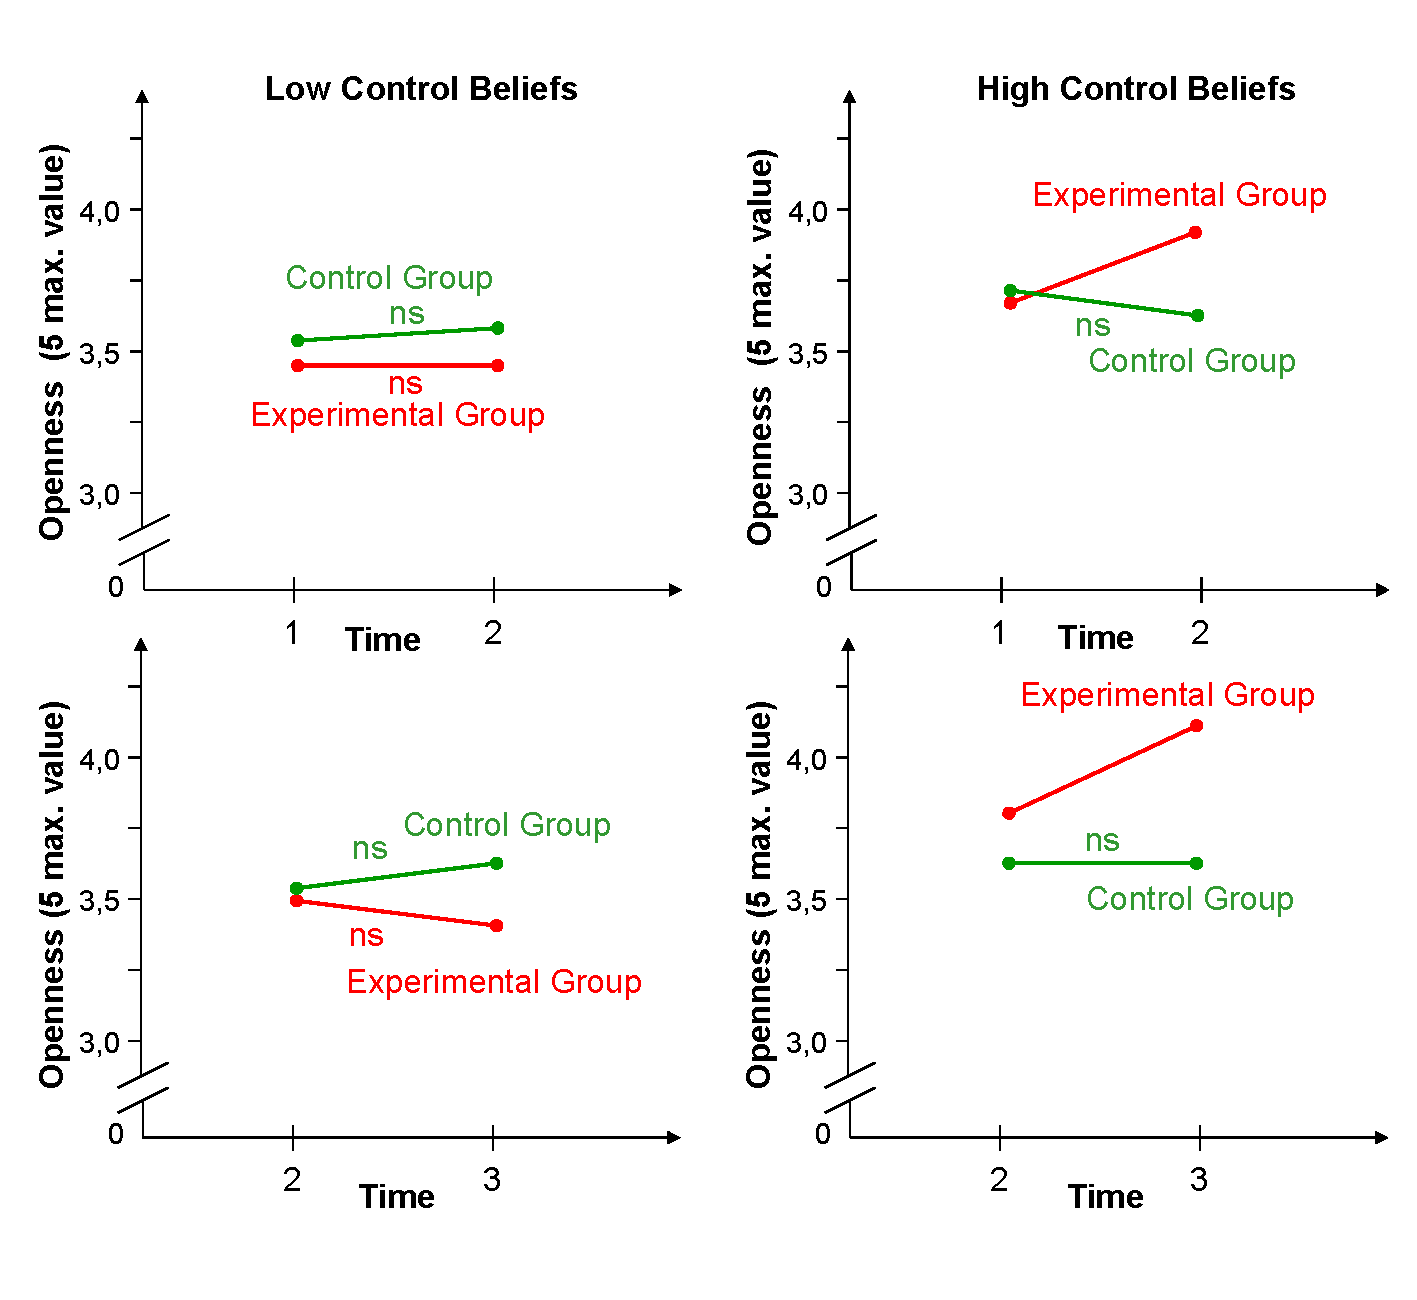
\includegraphics{profUrsulaStaudinger-fig3}}
    \caption{For participants with above median levels of internal control beliefs, the participation in the EFI program resulted in increases in Openness to Experiences. These increases were sustained across a period of 12 months (M\"uhlig-Versen \& Staudinger, in preparation).}
    \label{fig3:profUrsulaStaudinger}
  \end{center}
\end{figure}

\newpage

 All in all, the study shows that most likely it is not enough to become active to feel better but rather that specific circumstances, such as skill training and/or self-determination, need to be attended to as well.
 
\textit{The Effects of the Work Context on Adult Development}

 This is a new area of research that has started to emerge over the last year. One aspect that is of interest here is the effect of aging stereotypes present at the workplace on productivity and well being of older workers. First insights were gained from a JCLL pilot study that was conducted in the context of the Executive Master Program on Aging Workforce Management (LKI). In a sample of about 600 employees from 10 companies, we found as expected that older employees of companies with a rather negative aging stereotype showed poorer self-regulation as well as poorer job performance.


\paragraph{Collaborations}

\begin{itemize}
\item Deutsches Zentrum f\"ur Altersfragen DZA, Berlin\\ Prof. Dr. Clemens Tesch-R\"omer
\item Kassel University\\ Prof. Dr. Ekkehard Frieling 
\item Bremen University\\ Prof. Dr. Johannes Huinink
\item Yale University\\ Prof. Becca Levy, PhD
\end{itemize}

\begin{bibunit}[apalike]
\nocite{*}
\putbib[profUrsulaStaudinger3]
\end{bibunit}

\enlargethispage{2cm}
\paragraph{Grants}
\begin{itemize}
\item DFG STA 540/5 - 1/2 (PI: U.M. Staudinger): Age-heterogeneous interaction as facilitative developmental context (2003-2006).
\item BMFSFJ (PI: U.M. Staudinger): Personality development in old age: A natural intervention study (2001-2006).
\item Leopoldina (PI: U.M. Staudinger): Leotech Aging: Network that investigates Aging, Education and Work (2006-2009).
\item BMBF (PI: JCLL). U.M. Staudinger, U. Kunzmann: subproject ``Images of Aging'' within the joint research project ``Effects of Matches/Mismatches between Aspects of Human and Social Capital, Corporate Strategy and Work Organization on the Physical and Mental Well-Being of Employees''. 
\item DFG Travel Grant for Eva-Marie Kessler for Gerontological Society of America Annual Meeting 2006
\end{itemize}


\newpage
\subsection{Plasticity and Positive Development: Theoretical and
Empirical Approaches}



\index{Staudinger, M. Ursula}

\paragraph{Research Team}
Ursula M. Staudinger (Professor), Jessica D\"orner (Doctoral Fellow until 05/2006), Eva-Marie Kessler (Doctoral Fellow, graduated in January 2006; now Postdoctoral Fellow)

Human development is not determined but plastic. This is one the central contentions of lifespan psychology. Based on biological, psychological and external resources any observed development trajectory can be changed within limits. Such changes can be directed towards an improvement or a deterioration of the normally observed developmental course. It is argued that it is theoretically and empirically useful to distinguish these two kinds of plasticity. In conjunction with negative deviations from the normal developmental course the concept of resilience has been introduced into the literature. It refers to the maintenance or regaining of normal levels of functioning in the face of stressors. In contrast, positive deviations from the developmental trajectory should be subsumed under the notion of growth. When considering development as such, rather than positive or negative deviations from an expected developmental course, it again may be meaningful to differentiate between two kinds of positive developments. One is primarily geared towards the achievement of growth and the other towards adjustment. This latter distinction has been a focus of our work in 2005.

\null
\textbf{Research Highlights 2006}

Does personality stay stable after young adulthood or is there continued change throughout middle and later adulthood? For decades, this question caused heated debate. Over the last couple of years, a consensus has emerged based on recent cross-cultural as well as longitudinal evidence. This consensus confirms that indeed there is personality change in middle and later adulthood. Many authors have labeled this change personality maturation or growth. In somewhat simplified terms the observed pattern is as follows: Neuroticism declines, conscientiousness and agreeableness increase. At the same time it has been argued that this pattern of personality change is the result of coping with the developmental tasks of adulthood and thus increased adjustment. We critically examined this practice of equating developmental adjustment with growth and pointed to the necessity of defining personality growth by reference to theories of personality development as well as lifespan theory. 

\paragraph{Collaborations}

\begin{itemize}
\item Universit\"at Hildesheim\\ Prof. Dr. Werner Greve
\item University Trier\\ Prof. Dr. Sigrun-Heide Filipp
\item IUB, JCLL\\ Prof. Dr. Ute Kunzmann
\end{itemize}

\hyphenation{Ent-wick-lungs-psycho-lo-gie Hassel-horn}
\begin{bibunit}[apalike]
\nocite{*}
\putbib[profUrsulaStaudinger4]
\end{bibunit}

\newpage
\subsection{Other Professional Activities}

\begin{itemize}
\item President elect German Psychological Association (DGPs).
\item Member of the Selection Committee of the Alexander von Humboldt Foundation.
\item Member and Vice-Chairperson of the Leopoldina and acatech Committee ``Aging-Work Education''. 
\item Senior Fellow of the International Network on Aging of the Max Planck Society (MAXNETAging).
\item Member of the Scientific Board of the German Center for Gerontology (DZA) in Berlin.
\item Member of Scientific Board Center Aging \& Work (Sloane Foundation).
\end{itemize}



\textit{Editorial Board Memberships}

Psychology and Aging (since 1997), Psychologie in Erziehung und Unterricht (since 2000), Psychologie Verlagsunion Book Series ``Psychologie-Forschung-Aktuell'' (2000-2005), Book Series Psychologische Diskurse (Verlag Vandenhoeck \& Ruprecht) (since 2003), Research in Human Development (since 2003), The Journal of Positive Psychology (since 2005), Developmental Science (since 2006).


